\documentclass[a4paper]{article}

%% Language and font encodings
\usepackage[english]{babel}
\usepackage[utf8x]{inputenc}
\usepackage[T1]{fontenc}
\usepackage[linesnumbered,lined,boxed,commentsnumbered]{algorithm2e}

%% Sets page size and margins
\usepackage[a4paper,top=3cm,bottom=2cm,left=3cm,right=3cm,marginparwidth=1.75cm]{geometry}

%% Useful packages
\usepackage{amsmath}
\usepackage{float}
\usepackage{graphicx}
\usepackage[colorinlistoftodos]{todonotes}
\usepackage[colorlinks=true, allcolors=blue]{hyperref}
\usepackage{subfig}
\usepackage{float}
\usepackage{amsmath}
\usepackage{caption}
\usepackage{adjustbox}

\title{Computer Vision: Incisor Segmentation}
\author{Thierry Deruyttere (r0660485) \& Armin Halilovic (r0679689)}

\begin{document}
\maketitle

\section{Introduction}
In this paper, we present our approach for automatic segmentation of incisor teeth in dental radiographs.
The approach mainly relies on ``Active Shape Modeling'', which is briefly explained in section \ref{sect:asm}.
Then, in section \ref{sect:preprocessing} we discuss how radiographs are preprocessed before model building and incisor detection is done.
Afterwards, we discuss two initialization methods we implemented in section \ref{sect:init-estimate}.
Section \ref{sect:evaluation} the formal performance evaluation procedure used for the results of the incisor segmentation process.
The experiments and results are be presented in \ref{sect:experiments}.
We also did some experiments with neural networks. They are discussed in section \ref{sect:nns}.
Finally, section \ref{sect:conclusion} provides a conclusion of the work done.

\section{Active Shape Modeling (ASM)}
\label{sect:asm}
The idea behind ASM is to create a statistical model for a certain object which can be used to segment said object in unseen examples. 
The way ASM does this is as follows.
To create such a model, training data is needed. 
The training data should consist of images combined with landmark annotations.
These landmark annotations consist of multiple points $({x_i, y_i})$ that indicate the object we want to recognize.
The full landmark can be represented as a vector 
\begin{equation}
\textnormal{\textbf{l}} = (x_1, y_1, x_2, y_2, \ldots, x_n, y_n)^T
\end{equation}
A problem with landmark annotations across different images, is that they are not necessarily all at the same position nor do they have the same scale or rotation.
\subsection{Generalized Procrustes Analysis (GPA)}
\bigskip
To cope with this problem we will first project all the landmarks into the same normalized coordinate system. 
We do this by using ``Generalized Procrustes Analysis''.
This algorithm can be seen in Algorithm \ref{algo:procr}.
\bigskip

\begin{algorithm}[H]
\SetKwData{Left}{left}\SetKwData{This}{this}\SetKwData{Up}{up}
\SetKwFunction{Union}{Union}\SetKwFunction{FindCompress}{FindCompress}
\SetKwInOut{Input}{input}\SetKwInOut{Output}{output}
\Input{A list of landmarks}
\Output{A list of normalized landmarks}
\BlankLine

\For{$l$ in landmarks}{
	$l$ $\leftarrow$ translate $l$ such that its origin is (0,0) by subtracting the mean\;
    $l$ $\leftarrow$ rescale $l$ such that it has a scale $1$\;
}
$ref$ $\leftarrow$ choose random reference landmark from landmarks\;
$converged \leftarrow false$\;
\While{not converged}{
	\For{$l$ in landmarks}{
    	$l$ $\leftarrow$ rotate $l$ towards $ref$\;
	}
$\bar{l}$ $\leftarrow$ calculate the mean landmark for all the landmarks\;
$d$ $\leftarrow$ distance between $\bar{l}$ and $ref$\;
$ref$ $\leftarrow$ $\bar{l}$\;
$converged \leftarrow d < threshold$\;
}
\Return{landmarks}
 \caption{Procrustes analysis}
 \label{algo:procr}
\end{algorithm}

\subsection{Principal Component Analysis (PCA)}
Once all the landmarks have been projected into a normalized coordinate system, ASM will apply PCA on these.
The result of this PCA will be two matrices containing the eigenvectors and eigenvalues.
To create the statistical model we will store the top-$k$ eigenvectors into a matrix $P$ and we will also save the mean landmark $\bar{l}$.
By doing this we can reconstruct a landmark $l$ with the following equations.
\begin{equation}
l \approx \bar{l} + Pb
\end{equation}
\begin{equation}
b = P^T (l - \bar{l})
\end{equation}
$b$ is also called the shape parameters.

\subsection{Matching the model on a new image}
When presented with a new image, we can apply the statistical model by first choosing an initial location where to put the model. 
How we derive this initial location can be read in section \ref{sect:init-estimate}.
Once this is done we look at a region around each point in this initial estimate.
For each of these regions we decide a better location for the current . 
How we look at a region and decide where to move a point can be read in the subsection below.

\cite{Cootes1992AnIT}.

\subsection{Grey level models}
Uitlegje


\section{Preprocessing}
\label{sect:preprocessing}
In order to improve the speed and efficiency of the segmentation process, images are preprocessed before they are used for model building and detection of teeth.

\subsection{Region of interest cropping}
First, to improve the speed of the whole process, images are cropped so that only the most relevant regions remain. This reduces the total preprocessing work that has to be done for radiograph.

All of the radiographs we received for this project looked very similar in a broad sense. 
The centers of the mouths always lied in a certain region of the image, and the scale was consistent across all images.
Because of this, we decided for the region of interest (ROI) to be a rectangle around the center of each image.
Since all images were similar, we have determined the exact location of the ROI experimentally.
The values were chosen so that the ROI for each of the images would contain each of the eight incisor teeth along with a small buffer around the teeth.
The values we set for the ROI rectangle were 
\begin{align} 
(x_{start}, y_{start}) &= (x_{mid} - 375, y_{mid} - 450) \\ 
(x_{end}, y_{end})     &= (x_{mid} + 375, y_{mid} + 700)
\end{align}
This results in a region of 750 by 1150 pixels. A drawback of this hardcoded approach is that a new radiograph which is shifted significantly will cause the segmentation process to not work correctly, since (a part of) the incisor teeth will then be cut off.

\subsection{Filters}
Filters have been used to make the teeth pop out more in the images.
This should aid in the model building and tooth detections steps.
If the difference between the teeth and the mouth tissues is large, grey level models should be much clearer at the edges of the teeth. 

Bilateral and CLAHE filters are applied on the images to ???? TODO: THIERRY PLS beetje uitleg over beide.
They are applied twice each in alternating turns, starting with the bilateral filter.

We have also considered the use of adaptive threshold filters and Sobel filters to increase the contrast between the teeth and the rest of the images or to make their edges much clearer, but did not manage to use and evaluate them in the time allocated to this project.

\subsection{Gaussian Pyramid}
\label{subsect:gaussian-pyramid}
For the implementation of a multi resolution search algorithm, a Gaussian pyramid of images is created.
This is a pyramid of a predetermined number of levels.
The pyramid starts at level 0, which contains the original image.
Each higher level then contains a downsampled image of the level before it using a Gaussian average.
Each pixel at a higher level contains a local average of a pixel neighborhood on the level below it in the pyramid.


Figure~\ref{fig:preprocessing} shows a radiograph after the preprocessing step.
\begin{figure}[!tbp]
    \centering
    \subfloat[]{{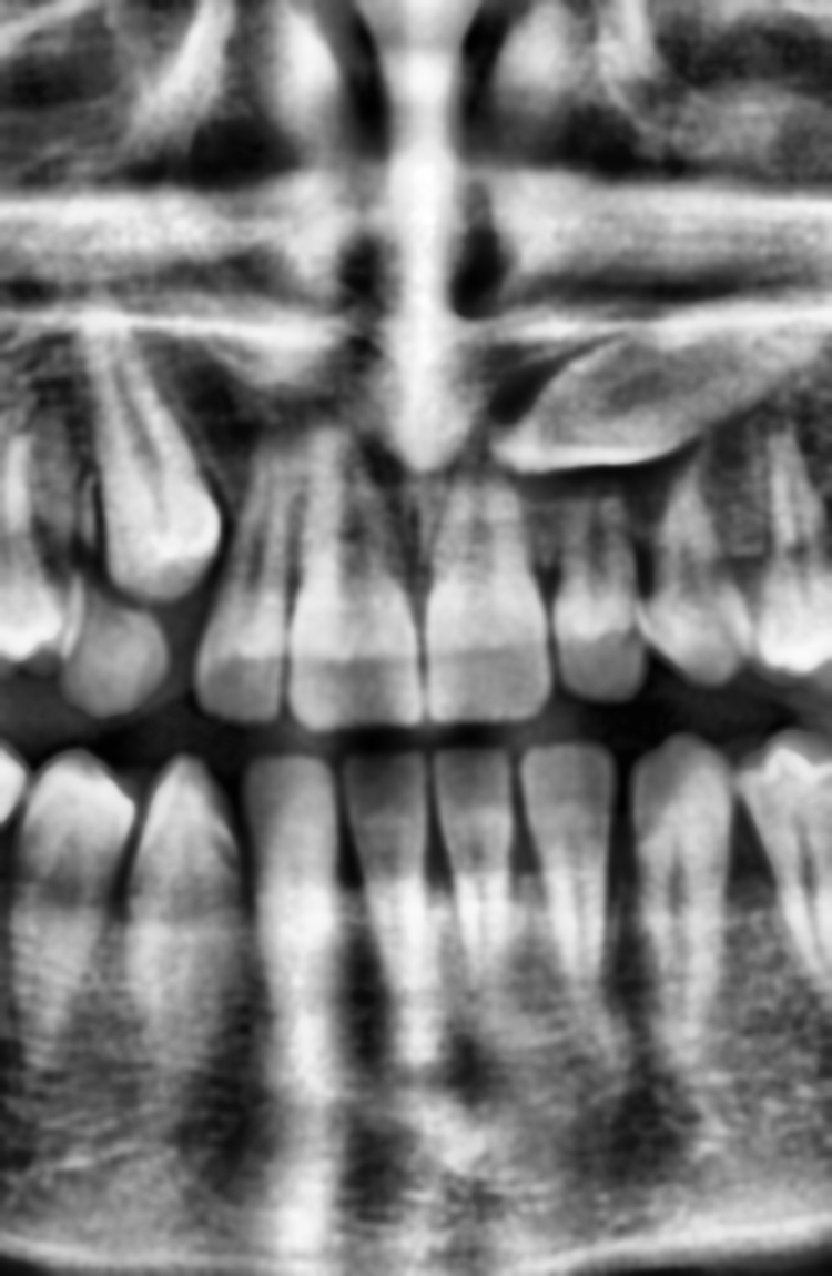
\includegraphics[width=5cm]{radiograph-01-preprocessed-level-0.png}}}
    \qquad
    \subfloat[]{{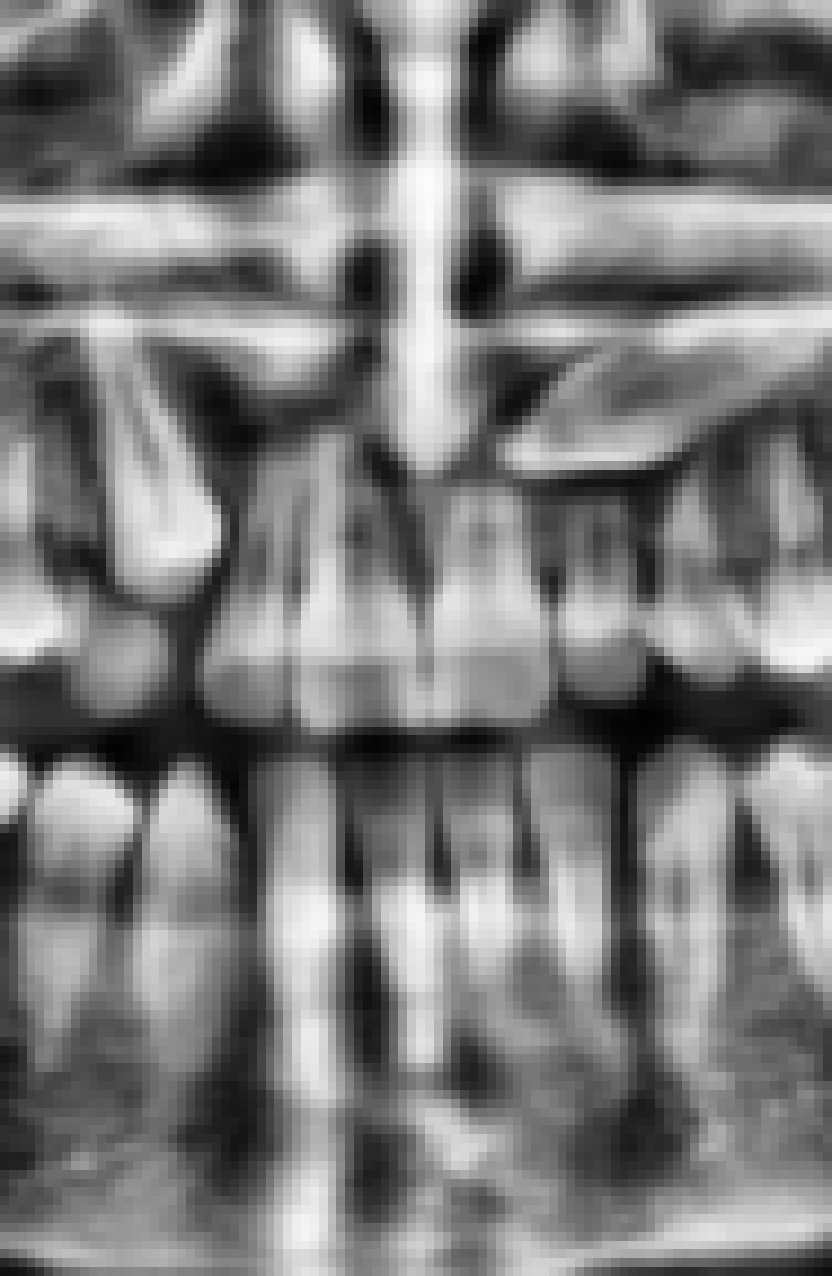
\includegraphics[width=5cm]{radiograph-01-preprocessed-level-3.png} }}
    \caption{Left, a radiograph (filename 01.tif) after the preprocessing step. Right, the same radiograph three levels higher in the Gaussian pyramid.}
  \label{fig:preprocessing}
\end{figure}

% \begin{figure}[!tbp]
%   \centering
%   \begin{minipage}[b]{0.48\textwidth}
%   	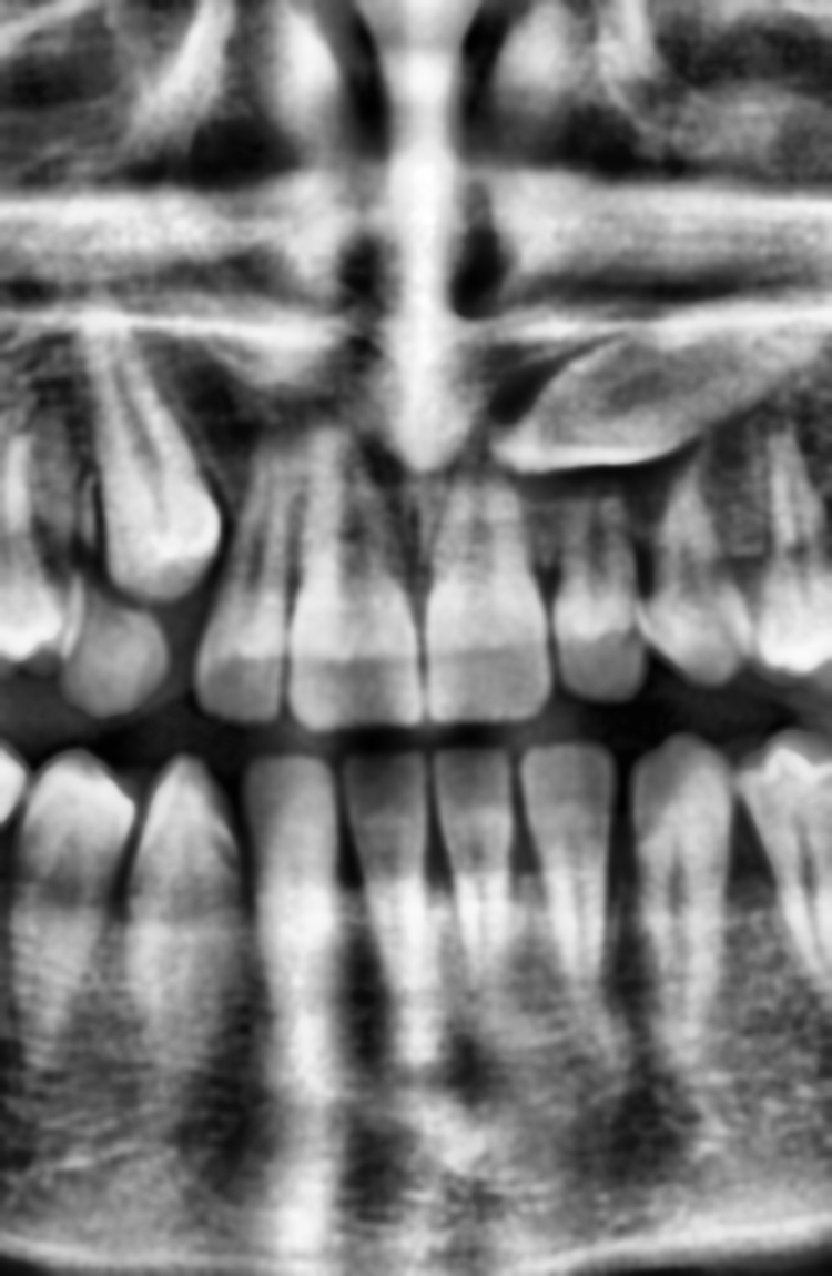
\includegraphics[width=\textwidth]{radiograph-01-preprocessed-level-0.png}
%   \end{minipage}
%   \hfill
%   \begin{minipage}[b]{0.48\textwidth}
%   	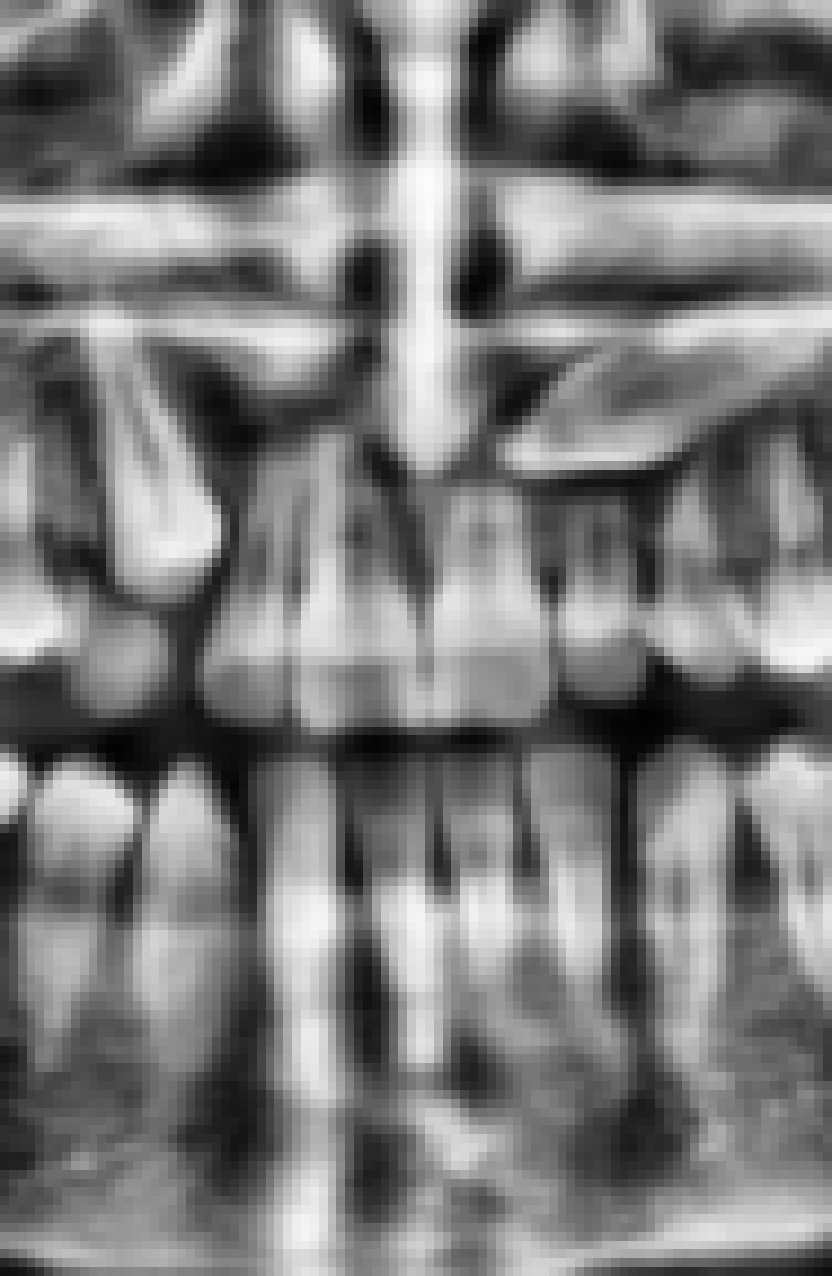
\includegraphics[width=\textwidth]{radiograph-01-preprocessed-level-3.png}
%   \end{minipage}
%   \caption{Left, a radiograph (filename 01.tif) after the preprocessing step. Right, the same radiograph three levels higher in the Gaussian pyramid.}
%   \label{fig:preprocessing}
% \end{figure}



\section{Fitting a model to an image}
\label{sect:init-estimate}
This section describes two approaches that were used for the fitting of an ASM.
The first method (subsection~\ref{subsect:upper-lower-incisors}) first goes through an initialization step based on an ASM for the upper four incisor teeth and another one for the lower four incisor teeth. When those models converge, individual teeth are segmented using models for individual teeth.
The second method (subsection~\ref{subsect:multi-res}) uses a multi resolution ASM for both the initialization and complete incisor detection.
Both of these methods rely on finding the center of the mouth for the initialization step, which is explained first.

\subsection{Locating the center of a mouth}
\label{subsect:center of mouth}
In order to find the vertical center of a mouth, a dynamic programming approach was implemented to find a path that can split the two jaws of the mouth. Since the area between two jaws is always black on the preprocessed radiographs, we opted to find a line that travels through this black area from left to right. Such a line, which we named the ``jaw split line'', is discovered by the Viterbi algorithm. 

The Viterbi algorithm was used to search for the darkest line in a region around the vertical center of each ROI. The algorithm is run on a region in the ROI to make the algorithm run faster and to not make it find lines at the top or bottom of ROIs. The search happens in a region described by the following variables:
\begin{align} 
y_{search\_min} &= y_{roi\_max} / 2 - 300\\ 
y_{search\_max} &= y_{roi\_max} / 2 + 200
\end{align}
The Viterbi search starts on the leftmost x position of each ROI with each of the y values in the region initialized to the intensity of the pixels in the ROI. The algorithm searches for the best path one x position at a time. For each next x position, it loops over each y position and looks at the best (i.e. lowest intensity) previous y position that can reach the current y position. The algorithm has been set to move forward in the path by 10 pixels at each iteration, and to look in a window of 10 previous y positions to find the next best y position. These settings make the algorithm run fast and find good jaw split lines.

Figure~\ref{fig:jawSplitLine} shows two jaw split lines. The left one is the split line in a relatively simple case; the black area between the jaws follows a fairly straight path. In the right one, the black area is not straight at all, but the Viterbi approach still manages to find a good jaw split line in this case.

\begin{figure}[!tbp]
    \centering
    \subfloat[]{{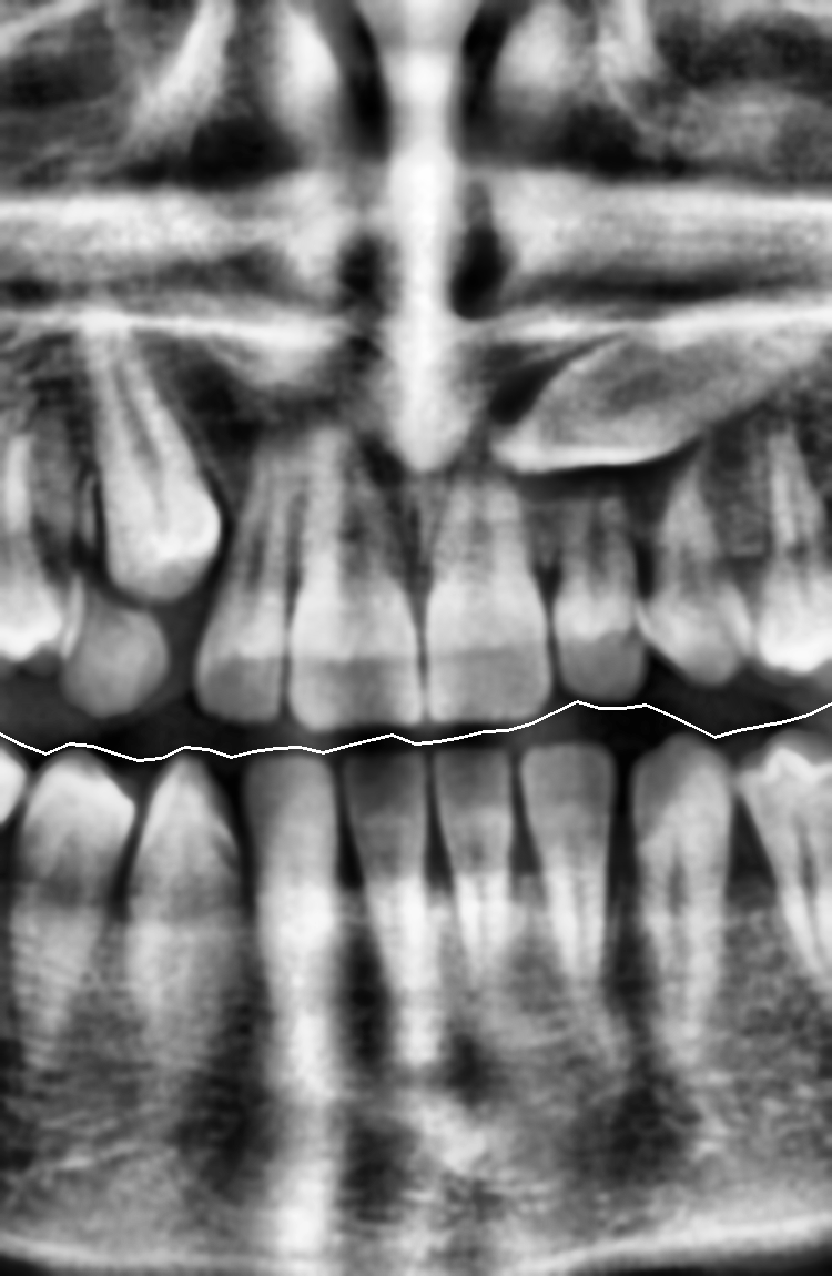
\includegraphics[width=5cm]{jawSplitLine-easy.png}}}
    \qquad
    \subfloat[]{{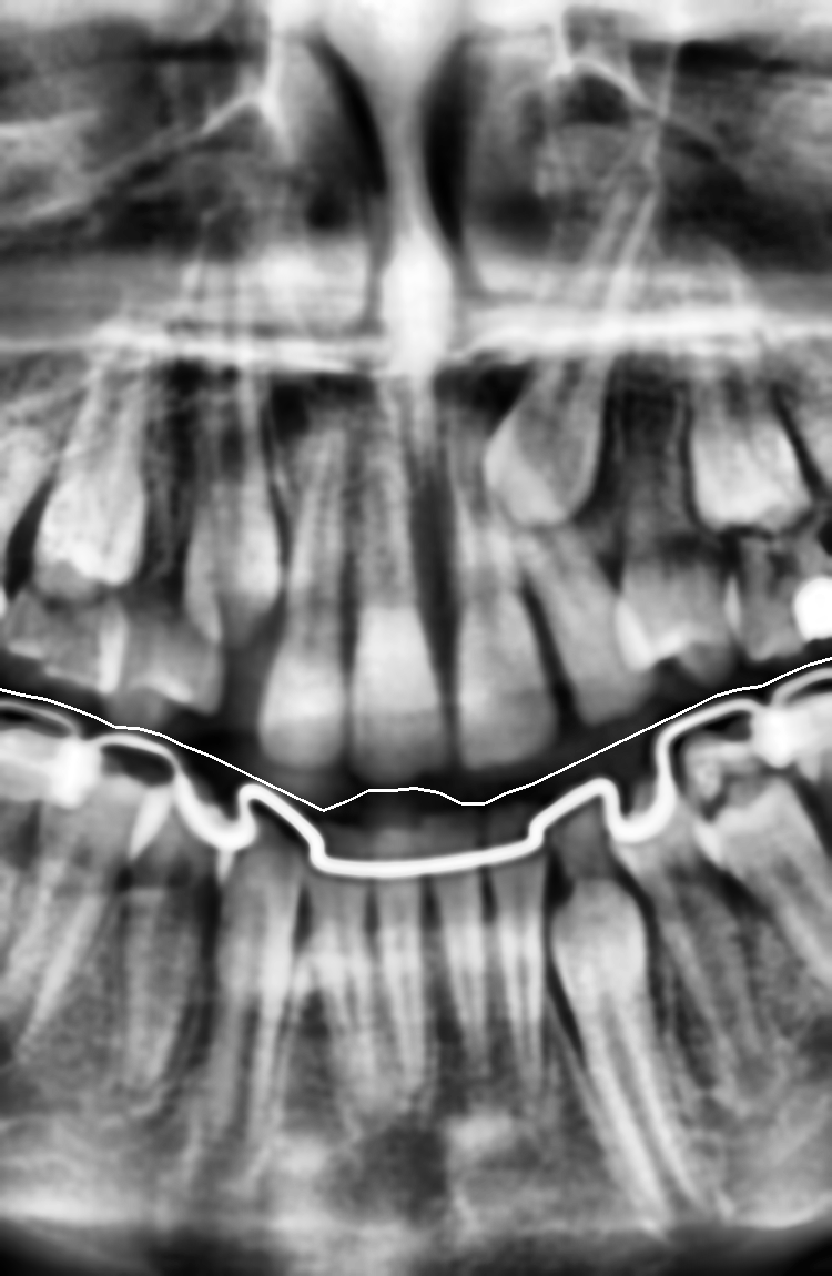
\includegraphics[width=5cm]{jawSplitLine-harder.png} }}
    \caption{Left, a simple jaw split line. Right, a more complicated one that follows the curve of the mouth.}
  \label{fig:jawSplitLine}
\end{figure}

% \begin{figure}[!tbp]
%   \centering
%   \begin{minipage}[b]{0.48\textwidth}
%   	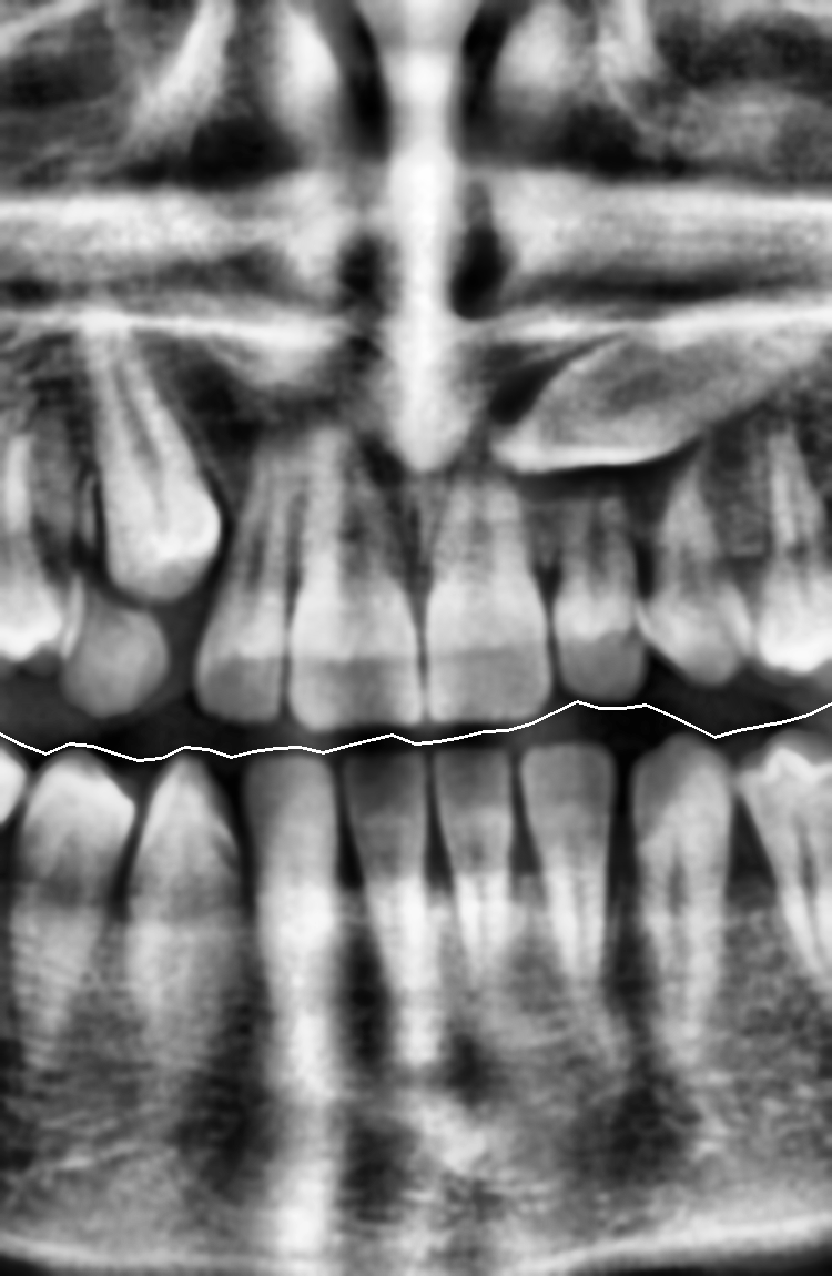
\includegraphics[width=\textwidth]{jawSplitLine-easy.png}
%   \end{minipage}
%   \hfill
%   \begin{minipage}[b]{0.48\textwidth}
%   	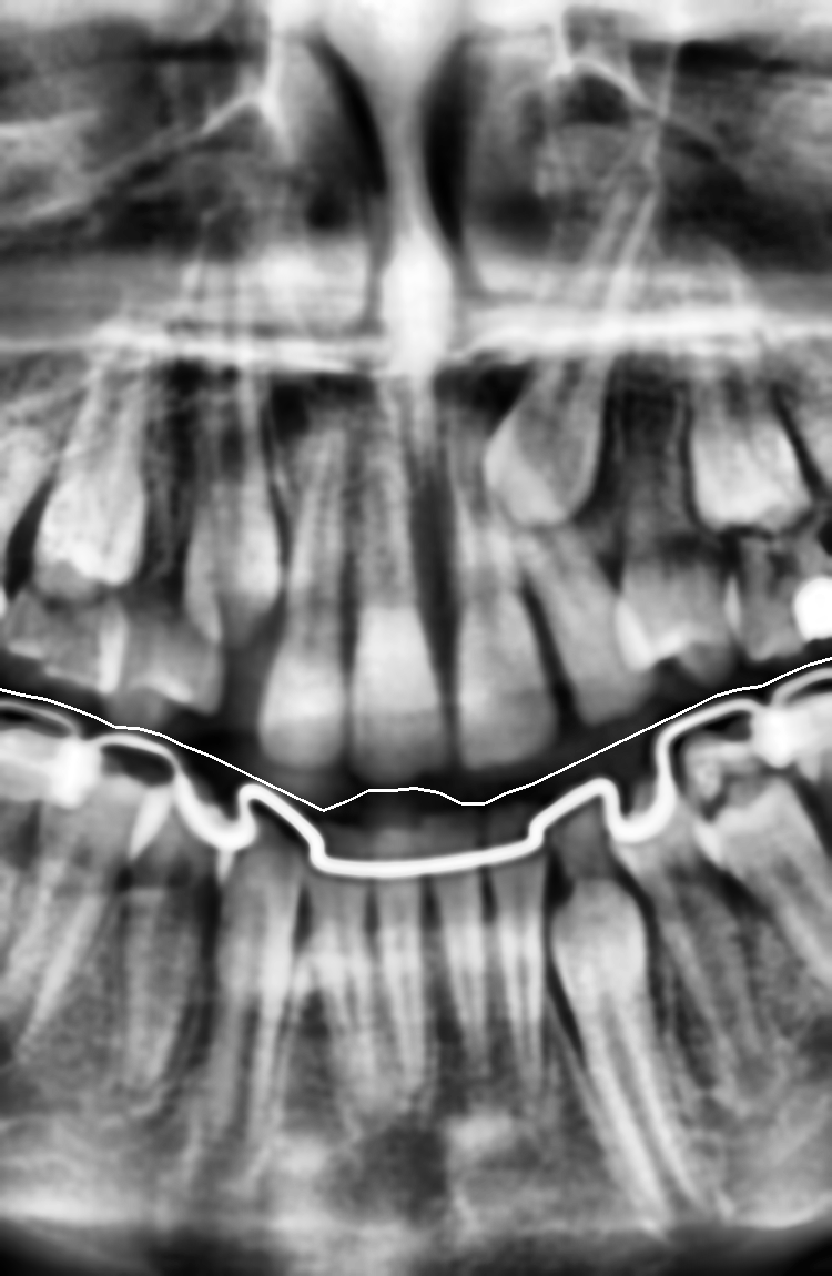
\includegraphics[width=\textwidth]{jawSplitLine-harder.png}
%   \end{minipage}
%   \caption{Left, a simple jaw split line. Right, a more complicated one that follows the curve of the mouth.}
%   \label{fig:jawSplitLine}
% \end{figure}

The horizontal center of each mouth is simply approximated by the middle x position of the ROI. This means that the horizontal centers will not be accurate for regions of interest in which the mouth is shifted significantly to the left or to the right. However, we noticed that most of the radiographs are nicely centered horizontally, which makes the middle x position .
Furthermore, the multi resolution search approach described in subsection~\ref{subsect:multi-res} is able to shift active shape models both horizontally and vertically so that the models can still move to correct positions 

The vertical center of each mouth is approximated by the mean y value of the jaw split line. Note that in contrast to the horizontal center, simply approximating the vertical by the middle y position would be much less accurate. This can be seen in figure~\ref{fig:jawSplitLine}, the mean y position would be well above the vertical center of each mouth. Also the mean y value of the jaw split line is different for the two lines shown in the figure.

\subsection{Model for the upper and lower incisors}
\label{subsect:upper-lower-incisors}
Iets met twee models laten convergen ofzo en dan daar boven of onder intializatie van een tooth ASM

\subsection{Multi resolution ASM}
\label{subsect:multi-res}
A multi resolution search approach was also implemented as described in~\cite{Cootes1992AnIT}. 
An active shape model in this case is trained for all eight incisor teeth at once.
Landmarks thus consist of 320 landmark points ($40\ points \times 8\ teeth$).

TODO: finish deze text na eten

This approach relies on a Gaussian pyramid as described in subsection~\ref{subsect:gaussian-pyramid}. 
A Gaussian pyramid is built for each train and test image.
First, grey level models are trained for each landmark point at each resolution level in the pyramid. 
Procrustes analysis is performed to normalize the landmarks, and to find the mean landmark, scale, and rotation.
PCA is performed on the normalized landmarks
Then, the search procedure is started at the highest level (i.e. lowest resolution image) in the pyramid. 
A low resolution version of the trained mean landmark is placed at the center of the mouth (found by the approach described in subsection~\ref{subsect:center of mouth}).

The multi resolution search approach simplifies the initialization procedure. 
At the highest level of the Gaussian pyramid, small movements correspond to large movements at the lowest level. 
Therefore, small movements of a landmark placed on the lowest resolution image correspond to larger movements in lower levels which move the landmark to a broad initial position.
Movements in each lower level resemble smaller movements which fit the model more precisely to tooth edges.

Figure~\ref{fig:multi-resolution-search-example} shows an example of this search procedure applied to the radiograph with filename ``24.tif''. This radiograph has no landmarks and thus was not used in the training of the model used for incisor detection. Figure (a) shows the start of the search procedure, with the white polygons representing the mean landmark placed on the detected center of the mouth. As described above, the procedure is started at the highest resolution level in the Gaussian pyramid. (b) shows the same landmark after it has converged on the highest resolution level. Then the landmark is scaled up (all points multiplied by 2) so it can be put on the level under it in the pyramid. The landmark is iteratively made to converge at a resolution level and moved to the lower until the lowest level is reached. (c) shows the same landmark that has converged on the original radiograph image.

\begin{figure}[!tbp]
  \centering
  \begin{adjustbox}{center}
    \subfloat[]{{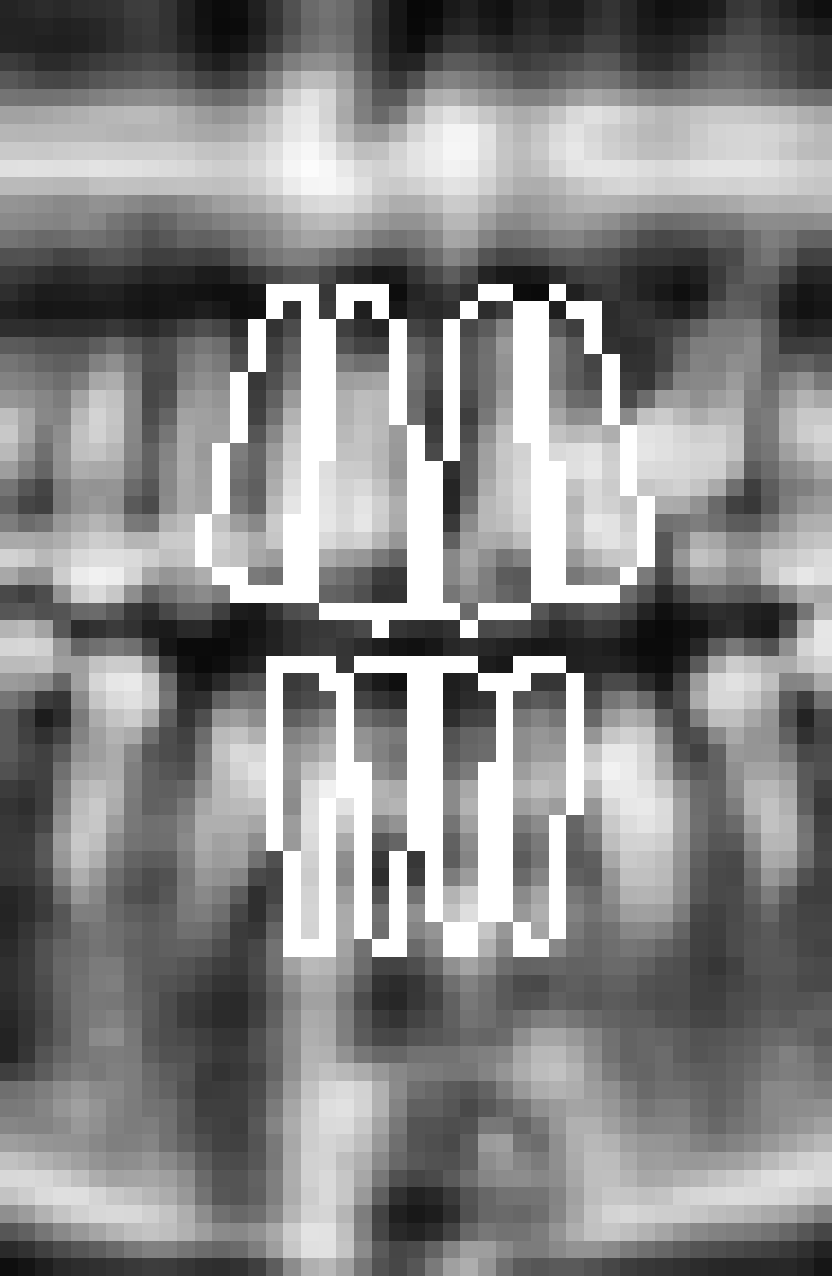
\includegraphics[width=5.5cm]{multi-resolution-24-init} }}
    \subfloat[]{{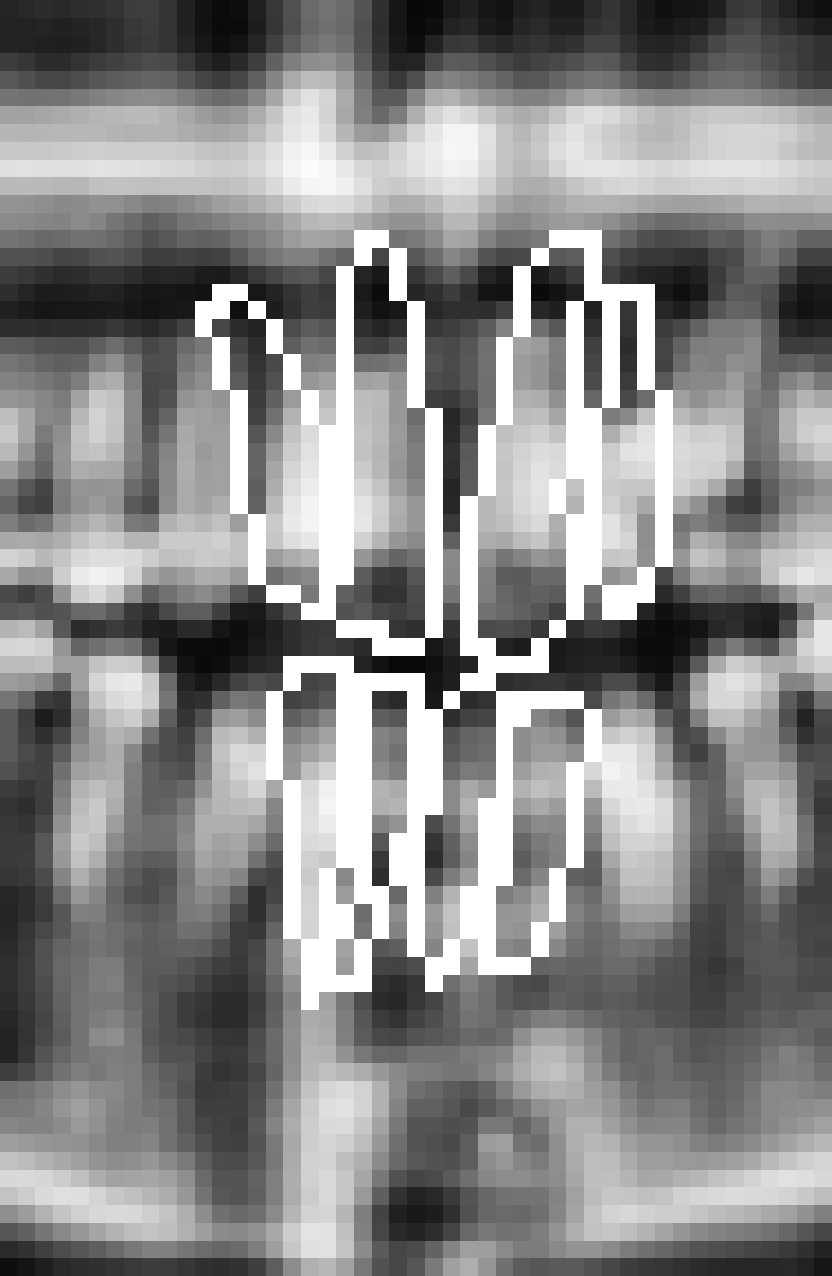
\includegraphics[width=5.5cm]{multi-resolution-24-init-converged} }}
    \subfloat[]{{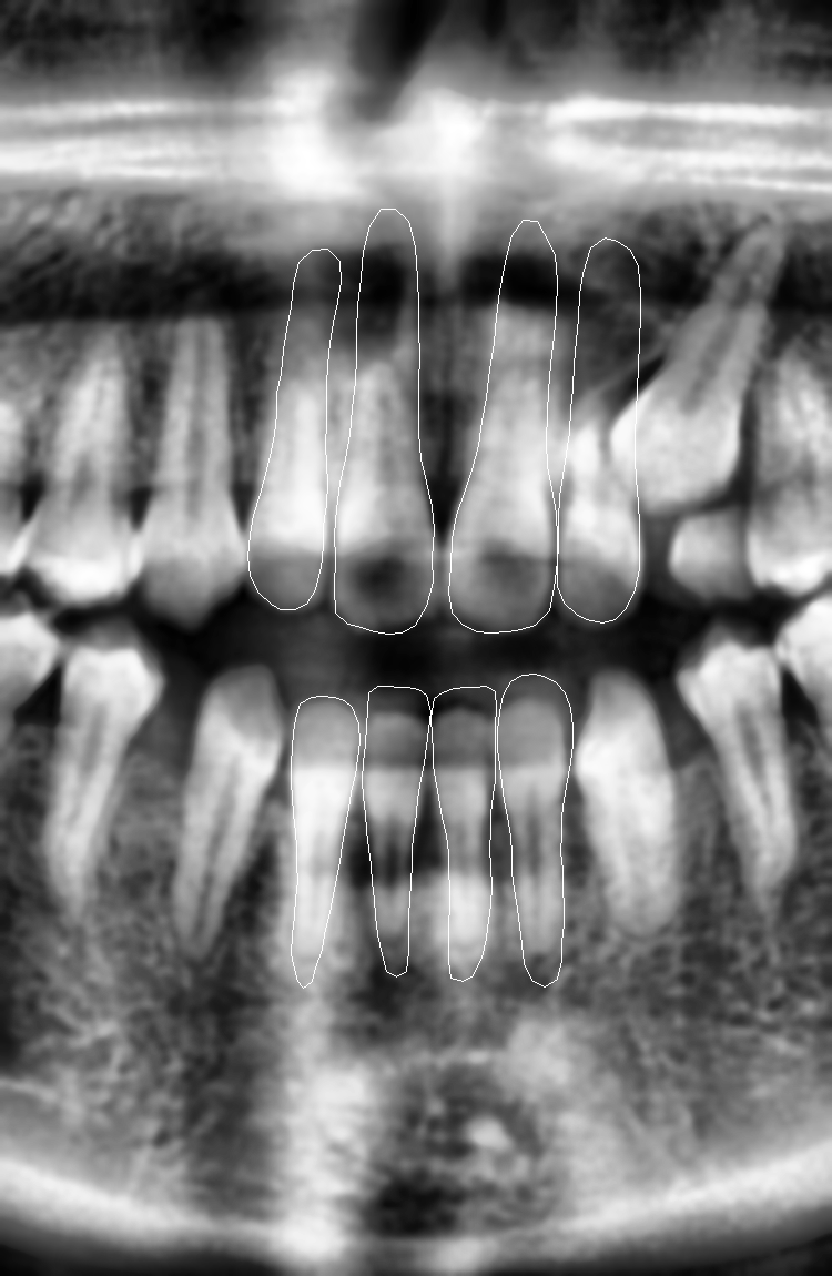
\includegraphics[width=5.5cm]{multi-resolution-24-final-converged} }}
  \end{adjustbox}
  \caption{The multi resolution ASM search approach applied to the radiograph with filename ``24.tif''.}
  \label{fig:multi-resolution-search-example}
\end{figure}

\subsubsection{PCA}
In this approach, landmarks consist of many more points than when modeling teeth individually. This posed a problem for the eigenvalues that were obtained after PCA was performed on the landmarks. Reconstructions of these landmarks were much less accurate and were more crinkly than smooth. An approach used to remedy this was to split the landmarks back up into eight landmarks and perform PCA for each tooth. Reconstructions were then made separately for each tooth and grouped back together into landmarks that contained all eight teeth. However, this cause teeth to overlap often, since the were reconstructed separately. A benefit of performing PCA on all teeth together is that the reconstructed landmarks then force the teeth to not overlap. Another approach to remedy this problem, the one that we ended up using, is to mirror all radiographs and their landmarks in order to double the training data. After performing PCA on the set of original and mirrored radiographs, reconstructions were much smoother, while still being able to adapt to new shapes found in improvement iterations, and still keeping teeth from overlapping.

\subsubsection{Parameters}
The following parameters were set for the multi resolution search experiments: \texttt{resolution levels} = 5, \texttt{maximum number of iterations allowed at each level} = 20, \texttt{number pixels on either side of point for grey level model} = 7, \texttt{number of sample points on either side of point for improvement search} = 3, \texttt{PCA components retained} = 25. 

These parameters were chosen based on subjective evaluation of performance. A better way to choose parameters would be by using a parameter optimization method such as grid search or Bayesian optimization.


\section{Evaluation}
\label{sect:evaluation}
Segmentations makes
TP, FP, TN, FN
accuracy, precision, recall


\section{Experiments}
Eerst zeggen dat we de foto's preprocessing met filters.
\label{sect:experiments}
\section{Neural Networks}
\label{sect:nns}

\section{Conclusion}
\label{sect:conclusion}

\newpage
\section{Appendix}
\label{sect:appendix}


\bibliographystyle{plain}
\bibliography{sample}

\end{document}